%!TEX root = ../../../main.tex
\section{Sensors and data processing} % (fold)
\label{sec:mr_sensors_and_data_processing}

	\subsection{Camera processing} % (fold)
	\label{sub:mr_camera_processing}
	In order to move around the robot workcells, a black line has been installed in the floor so it can be tracked.
	This line communicates the workcells themselves along with the internal parts of them. 
	These are: the entrance of the workcell, the conveyor and the position where the robot must place the processed order.
	To distinguish the areas QR codes have been placed in the floor following the convention that all the groups have agreed.

	Then, the camera sensor is used with two purposes:
	\begin{itemize}
		\item Detect the line
		\item Detect and read QR codes
	\end{itemize}

	\subsubsection{Line detection} % (fold)
	\label{ssub:line_detection}
	Speed and robustness have been the priority when designing the line detection.
	The filter works at 30 fps and with a extremely low failure rate.
	However, a inertia in the filter has been also added so this will return the last detected point during a certain time in case the line stopped being detected.

	Due to the line follower will adjust the PID given a reference point, the full image doesn't need to be interpreted.
	Because the reference point is going to be the center of the image (read section \ref{sub:mr_line_navigation}), the image is cropped with a vertical offset about the reference point.
	The width of the image is not cropped so the horizontal deviation can be measured in the largest range possible.
	After this crop, the image is binarized with an RGB threshold which give a robust detection of the black line.
	The line is then searched with a virtual horizontal line over the reference point.
	This line will cross with the black line giving two intersection points that, averaged, give the center of the line.

	In order to increase the robustness another 10 virtual lines are used equally with a vertical offset from the original line.
	The process is the same for them and the final point is the averaged one from the intersection points that are closer to themselves.
	This is done due to some noise can appear in the image (see figure \ref{fig:mr_camera_processing_2}) or a crossing line can be given (see figure \ref{fig:mr_camera_processing_3}).
	The 10 parallel lines (with a total accumulated offset bigger than the crossing line width) reduce the failure rate to the level of turning the filter into a very robust and fast enough filter.
	A clear representation is shown in the figure \ref{fig:mr_camera_processing_1}.

	The implementation has been carried out using the OpenCV libraries \cite{opencv}.
		\begin{figure}
	        \centering
	        \begin{subfigure}[ht!]{0.296\textwidth}
	            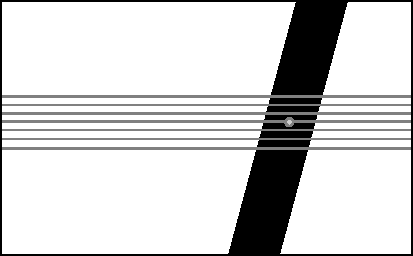
\includegraphics[width=\textwidth]{figs/mr_camera_processing_1}
	            \caption{Clear detection of the line}
	            \label{fig:mr_camera_processing_1}
	        \end{subfigure}
	        \hspace{40pt}
	        \begin{subfigure}[ht!]{0.296\textwidth}
	            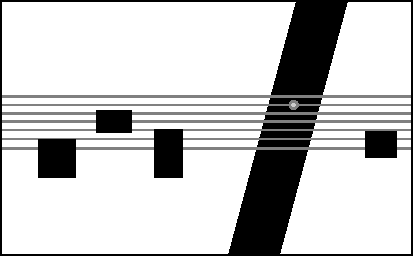
\includegraphics[width=\textwidth]{figs/mr_camera_processing_2}
	            \caption{Detection when noise in the image}
	            \label{fig:mr_camera_processing_2}
	    	\end{subfigure}
	    	\begin{subfigure}[ht!]{0.296\textwidth}
	            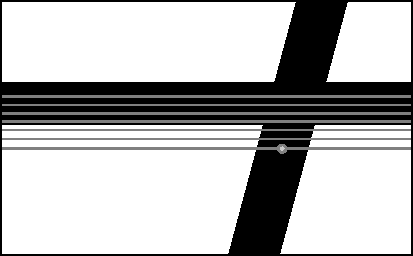
\includegraphics[width=\textwidth]{figs/mr_camera_processing_3}
	            \caption{Detection when crossing line}
	            \label{fig:mr_camera_processing_3}
	    	\end{subfigure}
	    \caption{Representation of possible cases when detecting the line}
	    \end{figure}
	% subsubsection line_detection (end)

	\subsubsection{QR detection and read} % (fold)
	\label{ssub:qr_detection_and_read}
	Due to the QR detection is made when moving, the image suffer a blur.
	This can be reduced with a Wiener motion noise filter but this is computationally expensive, so another approach has been taken.
	Instead, a fast shape detection is used, and if a rectangle of a determined size is detected, the speed is reduced until get a blur that doesn't affect to the QR reading.

	The QR detection is made by making use of the Zlib libraries \cite{zlib}. 
	These give you the ability of easily read the information contained in a QR code.
	% subsubsection qr_detection_and_read (end)


	% subsection camera_processing (end)

	\subsection{LIDAR processing} % (fold)
	\label{sub:mr_lidar_processing}
	\textbf{Martin + Dominik}

	% subsection lidar_processing (end)

	\subsection{Combined frobit odometry} % (fold)
	\label{sub:mr_combined_frobit_odometry}
	\textbf{Jorge}
	Wheels + IMU
	
	% subsection combined_frobit_odometry (end)

% section sensors_and_data_processing (end)